\documentclass[aspectratio=43]{beamer}

\usepackage[T1]{fontenc}
\usepackage[utf8x]{inputenc}
\usepackage[ngerman]{babel}
\usepackage{amsfonts,amsmath,amssymb,amsthm}
\usepackage{csquotes}

\usepackage{hyperref}

\usetheme[komms=false]{fbmathematik}

%%%%%%%%%%%%%%%%%%%%%%%%%%%%%%%%%%%%%%%%%%%%%%%%%%%%%%%%%%%
% Schriftfarben:
% tuklblau, tuklrot, warmgrau, kaltgrau;
% abgeschwächte Töne für die obigen Farben und schwarz:
% z.B. tuklblau7 für 70% tuklblau, warmgrau2 für 20%
% warmgrau oder schwarz6 für 60% schwarz,
% jeweils in den Schritten 10%, 20%, 40%, 60%, 70%, 80%;
% violette Schriftfarbe (Felix-Klein) hat den Namen fkz1
% hellviolette FKZ-Variante hat den Namen fkz2;
% KOMMS: kommsblau, kommsgruen, kommsgrau, kommsblaugrau
%%%%%%%%%%%%%%%%%%%%%%%%%%%%%%%%%%%%%%%%%%%%%%%%%%%%%%%%%%%



\title{Immer der Sonn' entgegen}
\subtitle{3. Zwischenbericht}
\author{Dominik Bendle \and Melissa Hasel \and Thomas Hofmann}
\date{\today}
\institute{TU Kaiserslautern}

\begin{document}

\begin{frame}[plain]

    % Leerzeilen vor und nach Titel sind offenbar nötig
    \Titel{logo}

\end{frame}

\begin{frame}
    \frametitle{Höhendaten reloaded}
    \begin{itemize}
        \item Modell mit Einbezug von Höhendaten wies in letzter Version Fehler auf
        \item[] $\rightarrow$ Fehler bei Einheitenumrechnung, Eingabe verfälscht
        \item Weiteres Problem: eher geringe Datendichte (ca.90\,m zwischen
            Koordinatenpunkten)
        \item vorherige Lösung: nimm nächstgelegenen Höhenwert
        \item jetzt: lineare Interpolation
        \item wegen besserer Funktionalität: auch ins OSM-Modell eingebaut
    \end{itemize}
\end{frame}

\begin{frame}
    \frametitle{Beispiele}
    \begin{figure}[t]
        \centering
        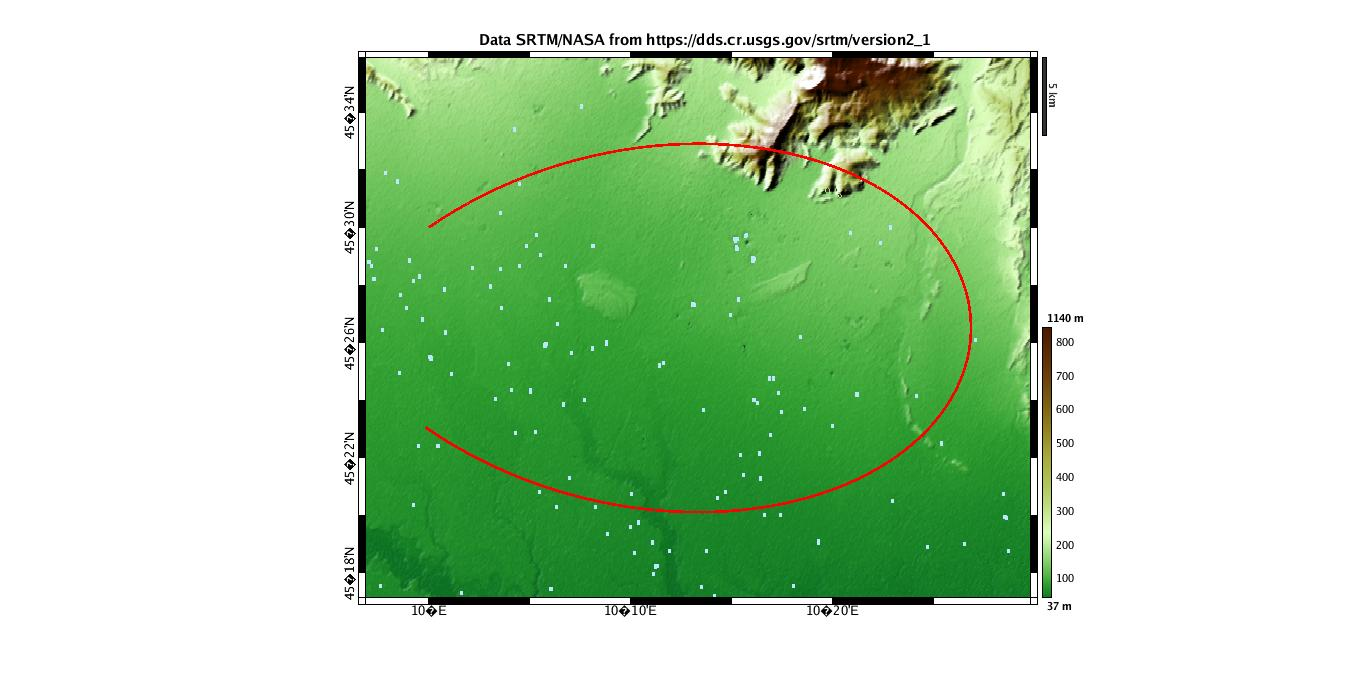
\includegraphics[width=0.95\textwidth]{bilder/nostreetnoele.jpg}
        \caption{Ohne Berücksichtigung der Höhe}
    \end{figure}
\end{frame}

\begin{frame}
    \frametitle{Beispiele}
    \begin{figure}[t]
        \centering
        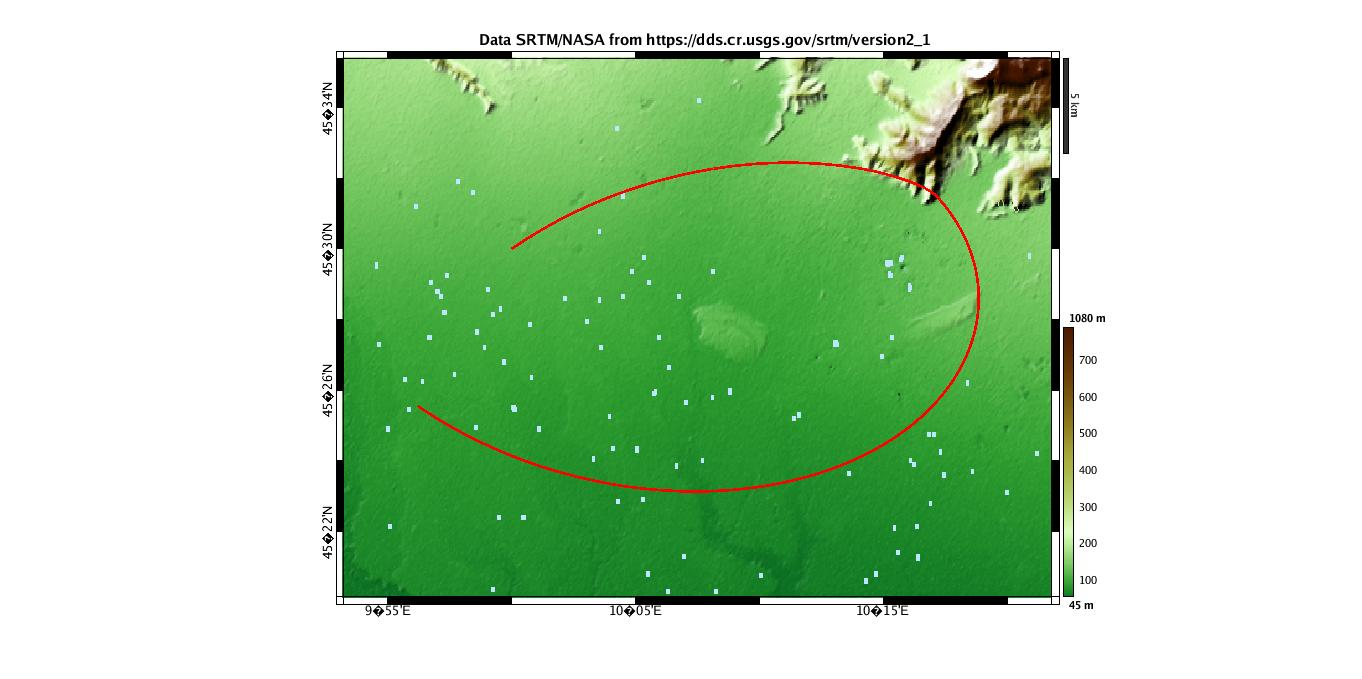
\includegraphics[width=0.95\textwidth]{bilder/nostreetele.jpg}
        \caption{Mit Berücksichtigung der Höhe}
    \end{figure}
\end{frame}

\begin{frame}
    \frametitle{Pausen und Laufgeschwindigkeit}
    \begin{itemize}
        \item bisher: den ganzen Tag lang gelaufen
        \item[] $\rightarrow$ für meiste Menschen unrealistisch
        \item können nun Lauf- und Pausenzeiten als \enquote{Fitness-Profil} an das Programm übergeben
        \item zusätzlich: Funktion, die Laufgeschwindigkeit in Abhängikeit von Zeit angibt
    \end{itemize}
\end{frame}

\begin{frame}
    \frametitle{Änderungen am Laufmodell (testweise)}
    Vorher
    \begin{itemize}
        \item An Kreuzung nimm gehe nur weiter wenn Straßen nicht von Sonne weg führen
        \item[] $\rightarrow$ bleiben in bestimmten Straßen für lange Zeit stecken
    \end{itemize}
    Nun
    \begin{itemize}
        \item wähle nun an einer Kreuzung immer einen Weg, auch wenn er von der Sonne
            wegführt
        \item mache nun niemals kehrt, d.h. gehe niemals in Richtung des zuletzt besuchten
            Knotens
    \end{itemize}
    Dies verhindert das Steckenbleiben in bestimmten Wegen, können aber dennoch in
    Rundwegen lange im Kreis laufen
\end{frame}

\begin{frame}
    \frametitle{Präsentation der Daten im OSM-Modell}
    \begin{itemize}
        \item gefundene route kann nun als Animation ausgegeben werden (Sackgassen,
            Rundläufe können besser nachvollzogen werden)
        \item haben zu Beginn zur Verdeutlichung der gefundenen Route die umliegenden
            Straßen geplottet, die in den Daten zur Verfügung standen
        \item[] $\rightarrow$ alle Straßen gleich dargestellt (wobei kein Problem der
            Daten, nur faule Implementierung)
        \item[] $\rightarrow$ Matlab-Plot enthält ggf. zehntausende Punkte und Linien und
            reagiert sehr langsam auf Interaktion
        \item entsprechend: animierte Ausgabe der Route teilweise sehr langsam
    \end{itemize}
\end{frame}

\begin{frame}
    \frametitle{Beispiel: Erste Darstellungsmethode}
    \begin{figure}[t]
        \centering
        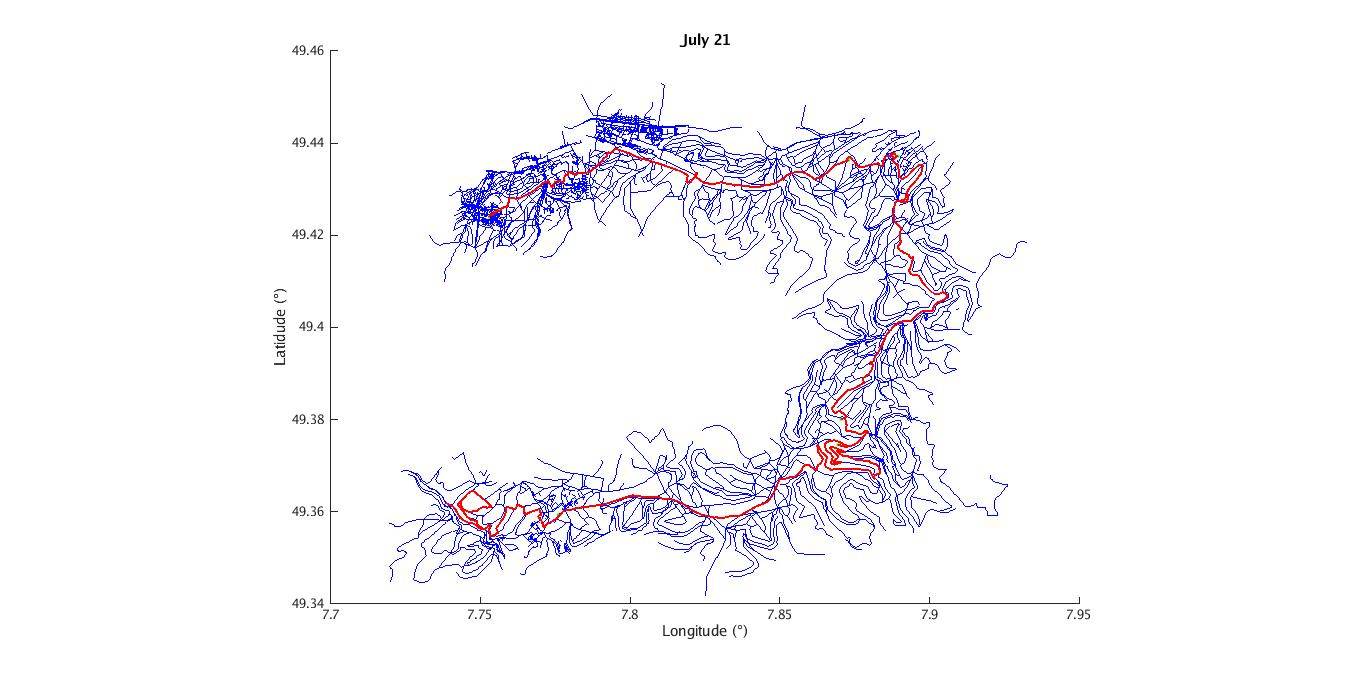
\includegraphics[width=0.98\textwidth]{bilder/lineele.jpg}
        \caption{Startpunkt TU-KL (mit Höhendaten, keine Pausen)}
    \end{figure}
\end{frame}

\begin{frame}
    \frametitle{Präsentation der Daten im OSM-Modell}
    Anderer Ansatz
    \begin{itemize}
        \item verwende Rastergrafiken bereitgestellt durch openstreetmap
        \item erste Idee: auf des finale Koordinatenrechteck zugeschnittene Grafik
            generieren lassen
        \item[] $\rightarrow$ kein Dienst bietet dies in automatisierbarer Weise an
        \item nächste Idee: OSM bietet Rastergrafiken in ca. 20 Zoom-Leveln als Kacheln an
        \item[] $\rightarrow$ berechne nötige Kacheln für fertige Route
        \item Problem bzw. fehlendes Feature: wähle richtiges Zoom-Level, um Ausgabe
            möglichst unverpixelt auszugeben (auch abghängig von Bildschirmauflösung)
    \end{itemize}
\end{frame}

\begin{frame}
    \frametitle{Beispiel: Neue Darstellungsmethode}
    \begin{figure}[t]
        \centering
        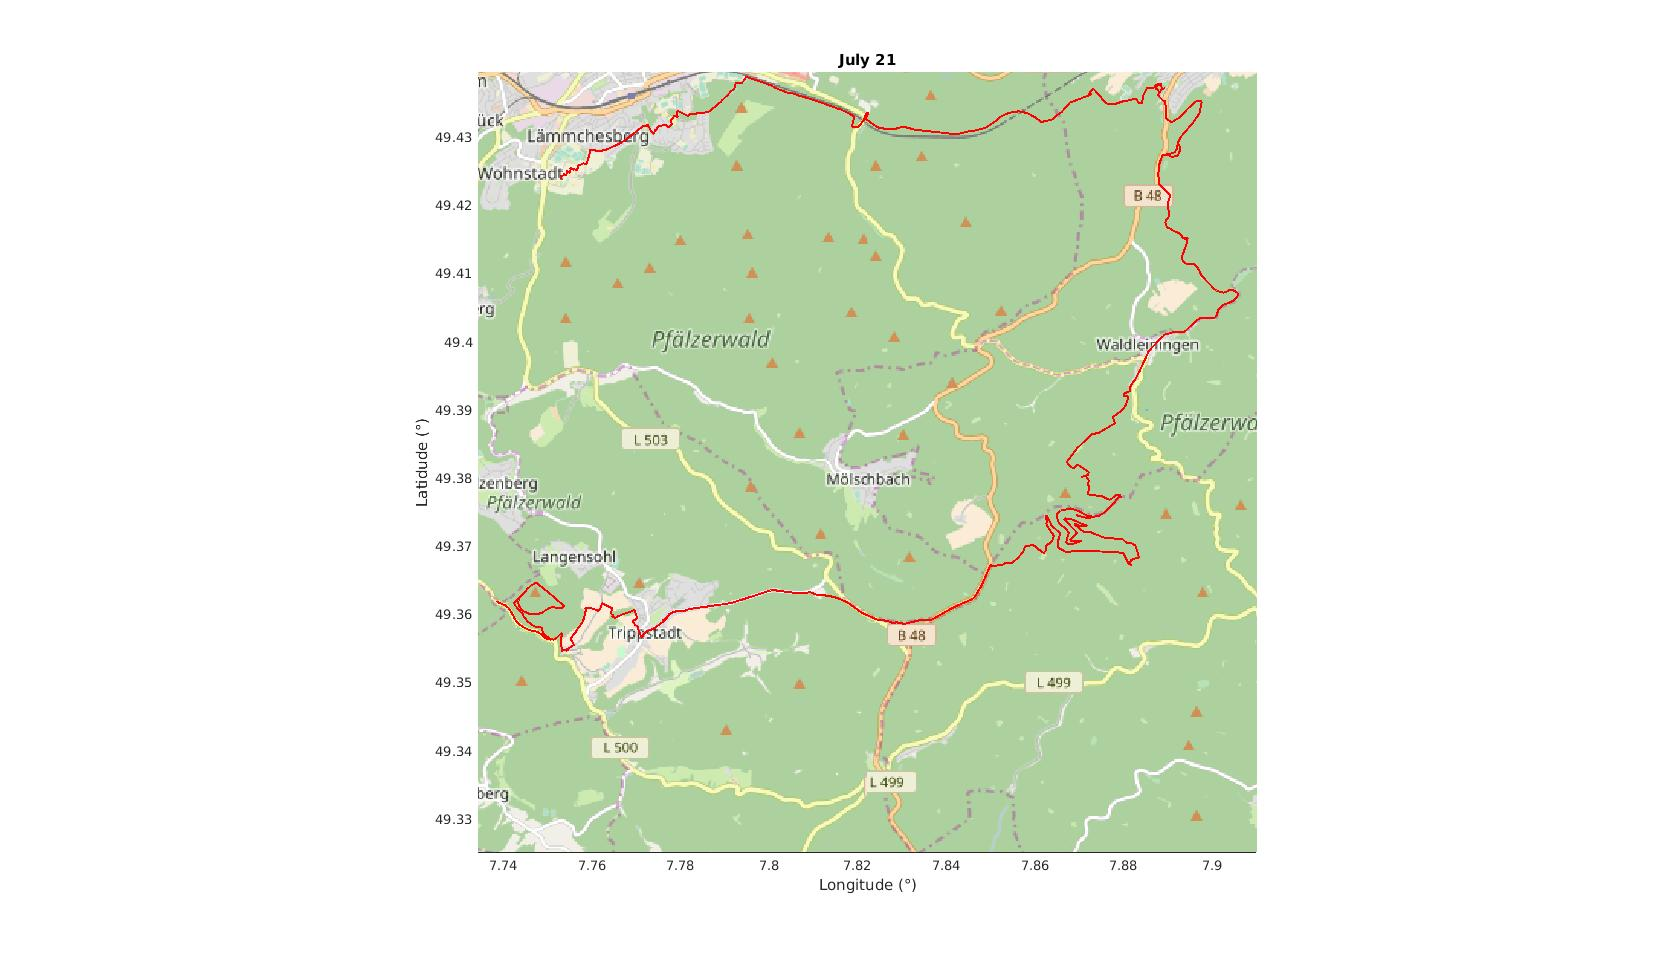
\includegraphics[width=0.98\textwidth]{bilder/ele.jpg}
        \caption{Gleiche Route}
    \end{figure}
\end{frame}

\begin{frame}
    \frametitle{Beispiel: Neue Darstellungsmethode}
    \begin{figure}[t]
        \centering
        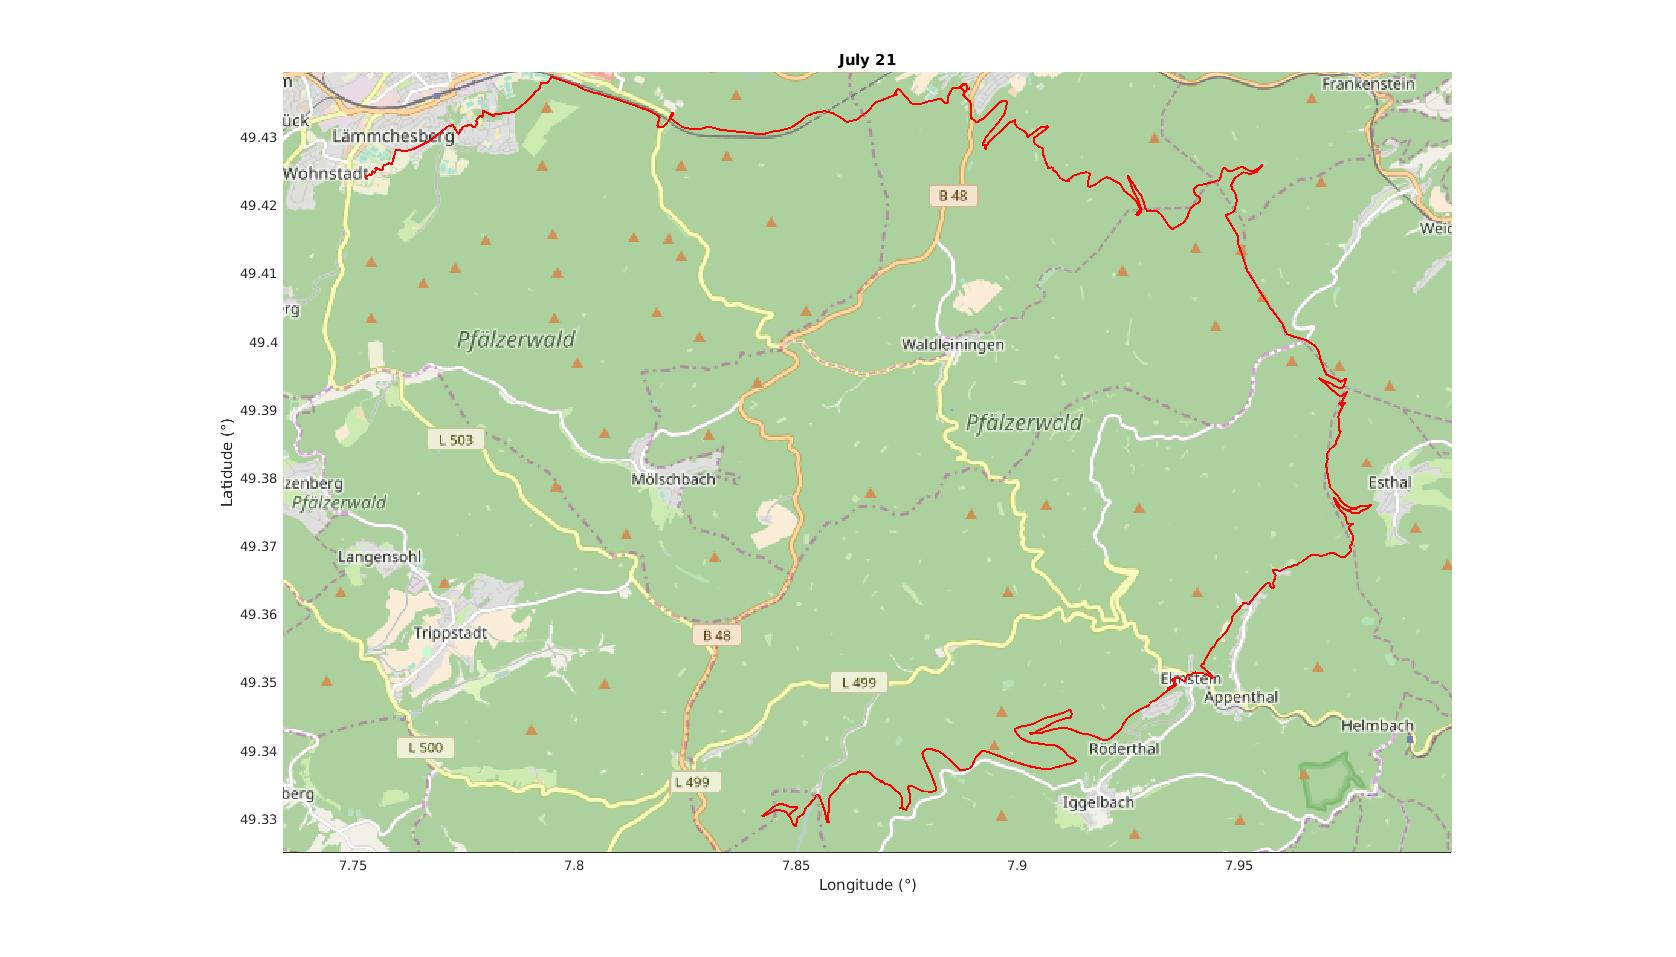
\includegraphics[width=0.98\textwidth]{bilder/noele.jpg}
        \caption{Diesmal ohne Berücksichtigung der Höhe}
    \end{figure}
\end{frame}

\begin{frame}
    \frametitle{Versuch: Modell von Straßen lösen}
    \begin{itemize}
        \item Idee: laufe ähnlich dem simplen Höhenmodell frei auf der Karte herum
        \item prüfe nach jedem Schritt, ob wir mit Objekt oder Barriere kollidieren;
            betrachtet werden z.Z. Gebäude, Barrieren, (breite) Flüsse, andere Ufer, \dots
        \item Kollisionsmodell funktioniert!
        \item erste Versuche, bei Kollision Auszeichen zu implementieren sind gescheitert
        \item weiteres Problem: Modell nur so gut wie die zugrundeliegenden Daten, in
            diesem Fall eher schlecht (unwegsames Gelände, dichte Hecken, etc. nicht
            modelliert)
    \end{itemize}
\end{frame}

\begin{frame}
    \frametitle{Weiteres Vorgehen}
    \begin{itemize}
        \item Vergleich unseres Sonnenmodells mit akkuraten Bestimmungsmethoden
        \item Verbesserung der Benutzerfreundlichkeit:
        \item[] $\rightarrow$ obige Arbeit mit Kacheldaten bietet Potential, den Benutzer
            via GUI Koordinaten wählen zu lassen
        \item Ausbau des straßenlosen Modells
    \end{itemize}
\end{frame}

\end{document}
